% !TEX root = ../thesis-example.tex
%
\chapter{Implementierung}
\label{sec:impl}
Dieses Kapitel beschreibt, wie das Konzept aus Kapitel \ref{sec:konzept} umgesetzt wurde. Es wird sowohl auf die neu implementierten Operatoren, als auch auf die verwendeten, bereits existenten RapidMiner-Operatoren eingegangen. 

\section{RapidMiner Studio}
\label{sec:impl:rms}

Die Plattform für das Parser-Framework wurde auf RapidMiner Studio \cite{rmstudio} festgelegt. Hierbei handelt es sich um eine Data Science Plattform, in der Operatoren im Steckkasten-Prinzip miteinander verbunden werden. Zwischen diesen Operatoren werden Daten in unterschiedlicher Form übergeben. Die Operatoren selbst führen verschiedene Aufgaben aus. Das eigentliche RapidMiner Studio bietet hauptsächlich Operatoren für die Verarbeitung von Tabellen an. Allerdings sind über den RapidMiner Marketplace auch eine Vielzahl von Erweiterungen erhältlich. Im Rahmen dieser Arbeit wird die Text Processing Extension (Version 8.1.0) \cite{textExt} %TODO ref text processing ext, ref https://rapidminer.com/products/studio/ 
verwendet. RapidMiner bietet zusätzlich die Möglichkeit eigene Operatoren zu programmieren, was im Rahmen dieser Arbeit auch genutzt wurde. Das RapidMiner Studio, die Erweiterungen und die eigenen Operatoren wurden in Java geschrieben. \\

\section{Verwendete Operatoren}

Hier werden die bereits bestehenden Operatoren beschrieben, welche im Prozess verwendet wurden.

Zum Einlesen des Parser-Modells wurde der Operator \textbf{Read File} aus dem Ordner \textit{Utility\textbackslash Files} verwendet. Dieser hat als Parameter den Pfad für die zu öffnende Datei. Er bietet einen Output-Port, über den die geöffnete Datei später als \texttt{com.rapidminer.operator.nio.file.SimpleFileObject} verarbeitet werden kann. Das Dateiformat der Modelle ist \textit{.bin} für den OpenNLP-Parser, \textit{.gr} für den Berkeley-Parser und \textit{.ser.gz} für den Stanford-Parser. Wichtig ist hier aber nicht die geöffnete Datei, da alle Parser diese selbst nochmal öffnen. Die Parser bekommen als Übergabe den Pfad und dieser kann aus dem \texttt{SimpleFileObject} entnommen werden.

Aus der Text-Processing-Extension wird der Operator \textbf{Read Document} verwendet. Er wird an zwei Stellen verwendet. Zum einen wird über ihn der Input-Text für den Parser eingelesen. Zum anderen wird der \textit{Goldstandard} für die Evaluierung damit in den Prozess gebracht. In beiden Fällen wird nur der Parameter \textit{file} auf den entsprechenden Dateipfad gesetzt und alle anderen Parameter auf ihrem Default-Wert belassen. Auch sein Input-Port wird nicht verwendet. Über den Output-Port wird die geöffnete Datei als \texttt{com.rapidminer.operator.text.Document} an die nachfolgenden Operatoren übergeben.

Der letzte verwendete Operator ist \textbf{Execute Script} aus dem Ordner \textit{Utility\textbackslash Scripting}. Dessen Aufgabe ist das Ausführen von Java Code. Verwendung findet er lediglich in Kombination mit dem Stanford-Parser. Die verwendeten Packages von Stanford werden hier einmal initialisiert, da es sonst einen Fehler seitens RapidMiner gibt. Hierfür wird ein Objekt der Klasse  \texttt{edu.stanford.nlp.trees.TreebankLanguagePack} erstellt und wieder auf \texttt{null} gesetzt. Weder die Input- noch die Output Ports des Operators werden genutzt, wodurch er vor den anderen Operatoren ausgeführt wird, und die Stanford-Packages korrekt initialisiert werden. Um diese Strategie der Fehlerumgehung nutzen zu können, sind zwei zusätzliche Schritte notwendig. Zum einen muss die Datei \textit{stanford-parser.jar}, welche die entsprechenden Packages beinhaltet, in den lib Ordner von RapidMiner Studio gelegt werden. Diesen findet man typischerweise unter \textit{Programme\textbackslash RapidMiner\textbackslash RapidMiner Studio\textbackslash  lib}. Das zweite und schwerwiegendere Problem ist der Bedarf einer Large License von RapidMiner. Mit der Lizenz in Kombination mit dem vorherigen Schritten wird der Fehler nicht geworfen. Anderweitig wird die Lizenz nicht benötigt. Für die Dauer dieser Arbeit wurde mir diese von RapidMiner kostenlos zur Verfügung gestellt.
\section{Eigene Operatoren}
\label{sec:impl:eigene}

Hier werden die Operatoren und alle dazugehörigen Klassen, die für dieses Parser-Framework entwickelt wurden, vorgestellt. 

Zur Entwicklung einer eigenen Erweiterung stellt RapidMiner eine Anleitung zur Verfügung \cite{rmguide}. %TODO ref https://docs.rapidminer.com/latest/developers/creating-your-own-extension/ 
Als Entwicklungsumgebung wurde Eclipse (Version: Oxygen.3a Release (4.7.3a)) in Kombination mit dem Gradle Plugin  gewählt. 

Alle entwickelten Operatoren erben von der Klasse \texttt{com.rapidminer.operator.Operator} und die Methode \texttt{doWork()} wird aufgerufen, wenn der Operator im Workflow durchlaufen wird. 

Die Übergabe von Daten zwischen Operatoren erfolgt über Klassen, die das Interface \texttt{com.rapidminer.operator.IOObject} implementieren, wie z.B. \texttt{ExampleSet} oder \texttt{Document}. 

Im Rahmen dieser Arbeit wurden folgende Operatoren erstellt: \textbf{Berkeley Parser}, \textbf{OpenNLP Parser}, \textbf{Stanford Parser}, \textbf{Compare Results} und \textbf{Show Results}

Alle Parser-Operatoren haben die gleichen Ports zur Ein- und Ausgabe. 
\begin{description}
\item[ioobjectInputGrammar]
Über diesen Port wird das Modell des Parsers eingelesen. Dieses wird in \texttt{doWork()} auf ein \texttt{SimpleFileObject} gecastet, um den Dateipfad auslesen zu können. Er wird mit dem Read-File-Operator verbunden.
\item[ioobjectInputText] Hier liest der Operator den Input-Text für den Parser ein. Das \texttt{IOObject} wird auf ein \texttt{Document} gecastet, um den Inhalt als String zu bekommen. Dieser String wird dann nach Zeilen getrennt, da jeder Parser immer eine Zeile eingegeben bekommt. Er wird mit dem Read-Document-Operator verbunden.
\item[nameOutputExt] Es wurde ein PortExtender verwendet. Das heißt, falls man diesen Port verbindet wird der selbe Port nochmals erstellt. Somit kann man die Parser Ausgabe öfters verwerten. Dies kann man z.B. nutzen, um in der Evaluation unterschiedliche Paramter zu setzen. Extender müssen im Konstruktor mit der Methode \texttt{start()} aktiviert werden. Über die von diesem Extender erstellten Ports wird der Name des Parsers in einem \texttt{Document} nach außen gegeben. Hierfür gibt es einen Konstruktor der Klasse Document dessen Übergabeparameter ein String ist. 
\item[resultOutputExt] Dieser Extender gibt den geparsten Text in einem \texttt{Document} aus. Hier sind alle einzeln verarbeiteten Zeilen wieder zu einem String zusammen gefügt worden.
\end{description}

\subsection{Berkeley-Parser}

Der Code für diesen Parser ist aus der Klasse \texttt{edu.berkeley.nlp.PCFGLA.BerkeleyParser} entnommen. Diese Klasse wird beim Kommandozeilenaufruf des Parsers angesprochen. Die \texttt{main}-Methode sowie \texttt{outputTrees(...)} wurden leicht abgewandelt übernommen. 

Die Funktionalität der \texttt{main} wurde in die \texttt{doWork()} geschrieben. Über den eigentlichen Kommandozeilenaufruf können Optionen übergeben werden, die in ein Objekt der Klasse \texttt{edu.berkeley.nlp.PCFGLA.BerkeleyParser.Options} geparst werden. Hier wird stattdessen ein Objekt dieser Klasse erstellt und die Optionen manuell gesetzt. Der Wert des Attributs \texttt{grFileName} wird auf den Dateipfad des eingelesenen Modells gesetzt. Bei allen anderen werden die Default-Werte beibehalten.\\ 
Die Ein- und Ausgabe in der Originalklasse war ein \texttt{BufferedReader} und ein \texttt{PrintWriter}. Das wurde abgewandelt, da die Eingabe jetzt zeilenweise als String zur Verfügung steht und die Ausgabe auch in einen String geschrieben werden soll. Der Parser bekommt seine Eingabe jetzt über eine \texttt{for}-Schleife, in der über das Array der Eingabesätze iteriert wird. Zuvor wurden per \texttt{while}-Schleife und die BufferedReader Methode \texttt{readLine()} der Parser-Input erhalten.

Die Methode \texttt{outputTrees(...)} wurde als Methode des Operators aufgenommen. Hierzu wurde der Rückgabetyp von \texttt{void} auf \texttt{String} geändert und der Übergabeparameter zur Datenausgabe von \texttt{PrintWriter} auf \texttt{String} abgeändert. Das führt dazu, dass statt \texttt{outputData.write("...")} nun \texttt{outputText += "..."} verwendet wird. Außerdem wird die Möglichkeit, die Ausgabe als .png zu erhalten, entfernt. Zuletzt wird der Methode ein \texttt{return outputText} angehängt. In der \texttt{doWork()} wird dieser String als \texttt{Document} verpackt und über den PortExtender an die Output-Ports geliefert.

\subsection{OpenNLP-Parser}
\label{sec:impl:eigene:opennlp}

OpenNLP bietet eine Anleitung zum Integrieren des Parsers in eine Anwendung mit Hilfe seiner API. Zu finden unter \cite{openNlpManual}. %TODO ref http://opennlp.apache.org/docs/1.9.1/manual/opennlp.html#tools.parser
Der Code aus dieser Anleitung wurde in die \texttt{doWork()} des Operator geschrieben. Dieser Code wurde von einem zusätzlichen \texttt{try-catch}-Block umgeben, um eine \texttt{FileNotFoundException} zu fangen. Diese Exception wird beim Öffnen der Datei des Parser-Modells geworfen. Per \texttt{for}-Schleife werden die Sätze der Eingabe in den Parser geschickt. 

Über die String Methode \texttt{outputText.replaceAll("\textbackslash \textbackslash (TOP ", "( ");} wird das Startsymbol des Parsers entfernt. Um zu verhindern, dass das Auftreten des Wortes ``TOP'' im Eingabesatz gelöscht wird, wurde die Klammer mit in den regulären Ausdruck aufgenommen. Worte des Satzes haben in der Formatierung immer eine schließende Klammer nach sich, aber nie eine öffnende vorher.

\subsection{Stanford-Parser}

Beim Herunterladen des Parsers wird eine Demo-Klasse mitgeliefert, in welcher der Code zum Starten des Parsers aufgeführt wird. Hieraus wurden die notwendigen Befehle in die Methode \texttt{doWork()} des Operators übernommen. Zu beachten ist hier noch, dass der Parser den Satz nicht als \texttt{String} entgegen nimmt, sondern die Token des Satzes in einem \texttt{String}-Array.

Das Startsymbol dieses Parser lautet ``ROOT'' und wird analog zum OpenNLP-Parser aus \ref{sec:impl:eigene:opennlp} entfernt.

\subsection{Compare Results}

In diesem Operator findet die Evaluierung statt. Es wird die Ausgabe von genau einem Parser mit dem \textit{Goldstandard} verglichen und die Kennzahlen errechnet.

Hierzu gibt es drei Input-Ports, deren \texttt{IOObject} jeweils zu einem \texttt{Document} gecastet wird. Der erste Port erhält den Namen des Parsers, der zweite die Ausgabe der Parser und der dritte den \textit{Goldstandard}. Das Ergebnis wird in einem einzeiligen  \texttt{com.rapidminer.example.ExampleSet} ausgegeben. Dadurch kann man später mehrere Evaluierungen in einer Tabelle untereinander anzeigen lassen. 

Der Operator hat zwei \texttt{Boolean}-Parameter. \texttt{PARAMETER\_REMOVE\_SUFFIX} gibt an, ob den syntaktischen Tags die Suffixe entfernt werden sollen. Das heißt, dass NP-SBJ als NP gewertet wird. \texttt{PARAMETER\_COUNT\_ONLY\_SYNTACTIC\_TAGS} entscheidet ob alle Tags oder nur die syntaktischen in die Bewertung zählen. Die Parameter wurden entsprechend dem Extension Manual \cite{rmguide} %TODO ref extension manual 
erstellt. Default-Wert bezüglich der Suffixe ist \texttt{true} und bezüglich der syntaktischen Tags \texttt{false}.

Für die Evaluierung benötigt dieser Operator zwei zusätzliche Hilfsstrukturen. Zum einen das Enum \textbf{PennTag}. Hier sind alle Tags der Penn Treebank aufgelistet. Jedes Literal hat einen String als Attribut, der die Schreibweise angibt. Somit kann über die statische Methode \texttt{stringToPennTag(String s, boolean removeSuffix)} ein String auf ein Enum-Literal abgebildet werden. Hierzu werden alle Tags durchlaufen und deren Attribut mit dem Übergabestring verglichen. Das entsprechende Literal wird zurückgegeben. Für den Fall, dass dem String kein Tag entspricht, wird das zusätzlich eingeführte Literal \texttt{Empty}, mit leerem String als Attribut, zurückgegeben. Das passiert beispielsweise dann, wenn im Parser oder \textit{Goldstandard} zusätzliche Tags verwendet werden. Eine Konstituente, die als Typ \texttt{Empty} hat, wird immer als falsch gewertet. \texttt{removeSuffix} sorgt dafür, dass die Tags ab dem ersten Bindestrich abgeschnitten werden und somit nur das ursprüngliche betrachtet wird. \\
Zum anderen wird die Klasse \textbf{ParseTreeNode} verwendet. Ein Objekt dieser Klasse entspricht einer Konstituente aus Kapitel \ref{sec:konzept:eval}. Realisiert wurde dieses Konzept über ein \texttt{PennTag} und zwei \texttt{int} Membervariablen für den Typ und die Grenzen. Über die Methode \texttt{equals(Object obj)} wird getestet, ob sowohl Tag, als auch Grenzen des übergebenen \texttt{ParseTreeNodes} mit dem aufrufendem übereinstimmen. 

Der Operator selbst bedient sich wiederum zweier Hilfsmethoden. Mit 

\texttt{private static String formatSentence(String s)} 

wird jede Zeile so formatiert, dass vor und hinter jeder Klammer ein Leerzeichen ist. Außerdem gibt es keine aufeinanderfolgenden Leerzeichen. Dadurch kann der String nach Leerzeichen geteilt werden. Durch

\texttt{private static List<ParseTreeNode> parseSentence(String s, boolean removeSuffix, boolean countOnlySyntacticTags)}

wird eine formatierte Zeile \texttt{s} in eine Liste von Konstituenten umgewandelt. Hierfür wird ein \texttt{Stack<ParseTreeNode>} genutzt. Der Satz wird nach Leerzeichen in Klammern, Nichtterminale und Terminale aufgeteilt. Diese werden mit einer \texttt{for}-Schleife durchlaufen. Damit ergeben sich vier Fälle. 
\begin{itemize}
\item Fall 1: Öffnende Klammer. Es wird ein neuer \texttt{ParseTreeNode} erstellt und dessen Startpunkt auf die aktuelle Wortposition im Satz gesetzt. Diese Konstituente wird auf den Stack gelegt.
\item Fall 2: Nichtterminal. Die oberste Konstituente des Stacks wird geholt, ihr Typ auf das gelesene Nichtterminal gesetzt und sie selbst wieder auf den Stack zurückgelegt.
\item Fall 3: Terminal. Der Wortzähler wird inkrementiert. Das eigentliche Terminal wird nirgends abgespeichert, da diese in der Parser-Ausgabe und im \textit{Goldstandard} identisch sind. 
\item Fall 4: Schließende Klammer. Der oberste \texttt{ParseTreeNode} wird vom Stack geholt und sein Endpunkt auf den aktuellen Stand des Wortzählers gesetzt. Gilt \texttt{countOnlySyntacticTags == true}, so werden nur diejenigen \texttt{ParseTreeNodes} an die Ausgabe gehängt, deren \texttt{PennTag} zu den syntaktischen Tags gehört. Falls nicht, so wird jede Konstituente der Ausgabeliste hinzugefügt.
\end{itemize}
Diese Methode gibt alle zu bewertenden Konstituenten des Satzes zurück. 

In der \texttt{doWork()} des Operators werden sowohl Parser-Ausgabe, als auch \textit{Goldstandard} nach Zeilen aufgeteilt. Für jede Zeile der beiden Versionen werden die beschriebenen Hilfsmethoden aufgerufen. Die Parser-Konstituenten werden durchlaufen und im \textit{Goldstandard} nach passendem Gegenstück gesucht. Hierdurch bekommt man die Anzahl an korrekten Konstituenten. Für den \textit{RCB}-Wert werden nochmals die \texttt{ParseTreeNodes} des Parsers durchlaufen und alle gezählt, die mindestens eine Konstituente des \textit{Goldstandards} kreuzen. Diese beiden Zahlen, sowie die Anzahl an Parser- und \textit{Goldstandard}-Konstituenten werden für jede Zeile aufsummiert. Dadurch können, nach dem Vergleich aller Zeilen, entsprechend der Formeln (\ref{eqn:precision}) bis (\ref{eqn:rcb}), die Kennzahlen für den Parser errechnet werden. \\
Zuletzt wird ein \texttt{ExampleSet} mit den Attributen \texttt{Name, Precision, Recall, F1, Crossing Brackets}, sowie der totalen Anzahlen der Konstitueten, aus denen die Kennzahlen berechnet wurden, erstellt. Diese eine Zeile mit den Werten des Parser, wird in dieses Set eingefügt, welches dann an den OutputPort übergeben wird. 

\subsection{Show Results}

Dieser Operator dient lediglich dem Zusammenführen von mehreren Parser-Evaluationen. 

Es wird für die Input-Ports wieder ein PortExtender verwendet, um beliebig viele Compare-Results-Operatoren anschließen zu können. Der Output-Port liefert eine Tabelle, in der pro Zeile die Ergebnisse eines Parsers stehen.

In der \texttt{doWork()} werden alle Input-Ports durchlaufen und die Werte in die Ergebnistabelle übertragen. Diese wird zuletzt an den Output-Port geliefert.


\section{Prozess zum Evaluieren der Parser}

Mit den vorgestellten Operatoren lässt sich im RapidMiner Studio nun ein Prozess zum Evaluieren der Parser erstellen. Die Anordnung der Operatoren zur Evaluierung des Berkeley-Parsers wird in Abbildung \ref{fig:screenshot-prozess} präsentiert. Dieser Aufbau ist für alle Parser gleich. Lediglich bei \textbf{Read Grammar} muss beachtet werden, dass das entsprechende Modell geladen wird. Um mehrere Parser zu vergleichen,  muss das Konstrukt aus \textbf{Compare Results}, und allen links davon liegenden Operatoren, für die anderen Parser erstellt werden. Die Ausgänge der \textbf{Compare Results}-Operatoren werden mit \textbf{Show Results} verbunden. \\
Abbildung \ref{fig:results} zeigt einen Teil der Ausgabe des Prozesses beim Vergleich aller Parser. Nach dem Namen der Parser werden die vier Metriken aufgelistet. In der Abbildung wurden rechts vier Spalten entfernt, welche die Zahlen angeben, aus denen sich die Metriken berechnen. Diese Zahlen sollen unter anderem dabei helfen die Größe der geparsten Datei einzuordnen.

\begin{figure}
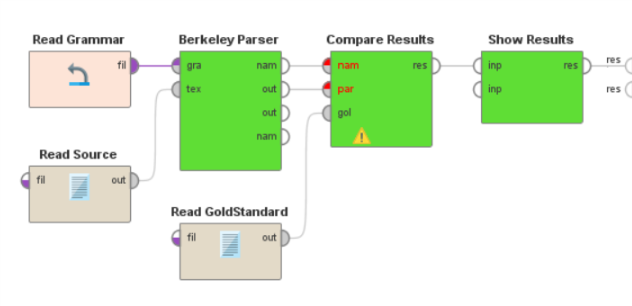
\includegraphics[width=\textwidth]{gfx/berkeley-skizze.png} 
\label{fig:screenshot-prozess}	
\caption{RapidMiner-Prozess zur Evaluierung des Berkeley-Parsers}	
\end{figure}

\begin{figure}
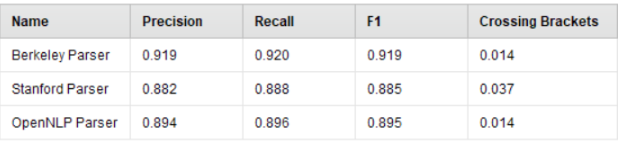
\includegraphics[width=\textwidth]{gfx/shortresults.png} 
\label{fig:results}	
\caption{Teil der Ausgabe des RapidMiner-Prozesses beim Vergleich aller Parser}	
\end{figure}